\section{Related Work}
\label{sec:searching:relwork}

The Web of Data consists of a wide range of heterogeneous datasets, where the schema and the ontology can vary from one to the other. To overcome this diversity of attributes, different approaches for defining the fields of an entity have been proposed.\\

From a RDF perspective, the authors consider in \cite{Perez-Aguera:2010:UBS} five weighted fields to represent the structure of an entity: literals (textual values), keywords extracted from the root's label, i.e., the subject URI, keywords extracted from the incoming links, the entity's types and keywords extracted from object URIs. Compared to the BM25F and PL2F field-based approaches defined in \ref{sec:ranking-wod}, this approach is not able to grasp the rich structure of the data since attributes are discarded.

The BM25F and PL2F approaches we use in our experiments Section~\ref{sec:experiments} are similar in nature to the BM25F adaptation proposed in \cite{blanco:2011:iswc}, where the authors consider one field per attribute in the data collection and can assign a different weight to each attribute. However, they restrict their approach to attributes with literal values, discarding those with URI values. In contrast to \cite{blanco:2011:iswc}, we consider attributes both with literal and URI values. URIs in a RDF graph carry relevant keywords, with regards to
\begin{inparaenum}[(1)]
	\item the entity in general when considering the subject URI;
	\item the attribute when considering the predicate URI; and
	\item the related entity when considering the object URI.\\
\end{inparaenum}
%We also consider in our approach the entity and the attribute labels, i.e., the predicate URIs, using special entity attributes. This aspect is discussed in the Section~\ref{sec:with-att}.

However, all these approaches are an adaptation of the field-based ranking model in which multiple values associated to a same attribute are aggregated into a single value. This simplification of the underlying data model is inadequate for structured data. Therefore, we propose an extension of field-based ranking models in Section~\ref{chap:tree-ranking:mf-model} to take into consideration multi-valued attributes and show that our model can be effectively applied to different ranking frameworks.

%\chapter{Ranking of (Semi-)Structured Data}
%
%At its beginning, The Internet was a collection of hypertext documents: textual data with links to additional textual data. At first, search engines were focused on retrieving documents, but with the growth of The Internet, a need for \emph{ranking} documents with regards to how important they are regarding a user's query appeared. Documents consisting only of text, the ranking models assumed as much and no structural information was considered. Nonetheless, some structural cues could still be extracted from the documents, e.g., title, paragraphs, links, \ldots, thanks to the HTML markup are written in. Including these cues into the ranking model improved noticeably its performance.
%
%With the coming of the Semantic Web, documents are turning into a real blend of structured and unstructured data. The structural information is clearly defined. Since this marked a shift of how documents are modelled, there was a need for ranking models to adapt. In this chapter, we present some ranking models used over (semi-)structured data, and introduce the ranking model used in this thesis as a basis for Chapter~\ref{chap:tree-ranking}.
%
%\section{Traditional Ranking Models}
%
%\section{Abstract Model}
%
%\section{Formal Model}

%\section{Entity Model}
%\label{chap:entity-ranking:entity-model}
%
%In this section, we define what is an entity, i.e., the unit of information that is queried and retrieved by an IR search engine. The entity model is based on the graph model presented in Section~\ref{sec:gdm:formal-model}.% In this chapter, we use \emph{document} as an equivalent term for \emph{entity}, since a document is the common term for the object that is ranked in an IR search engine.
%
%An entity in a graph data model is defined as a sub-graph in which a node is considered as the \emph{root}. In RDF the root is the URI that represents that entity, e.g., the URI \url{http://dbpedia.org/page/Earth} for referring to the planet Earth. The edges related to that root form then what we call an \emph{entity}.
%
%\begin{definition}[Entity]
%Let $G = \left\langle V, A, l_V \right\rangle$ be a graph. We call an entity rooted in $u \in V$ a sub-graph of $G$ in which the edges and nodes are a related to the root $u$.
%\end{definition}
%
%There exist several ways to define which edges are related to a root node. We can consider the entity as the connected component that emerges from that root. This can be achieved by performing a breadth-first search starting at the root, and adding the traversed edges and nodes to the entity. Also, one may consider a set of unconnected sub-graphs as the entity according to a similarity measure.
%
%In this chapter, we use the approach described in~\cite{delbru:jws:entity}, where an entity is a star graph, i.e., a sub-graph with a node (the root) and its direct neighbouring nodes it links to. The Figure~\ref{fig:rdf-graph} displays how a graph can be split into four entities \emph{me}, \emph{\_:b1}, \emph{\_:b2} and \emph{paper/547}. Each entity forms a sub-graph containing the incoming and outgoing edges of the root node. In order to simplify the extraction process, we only consider the outgoing edges of a root node.

%\subsubsection{Entity Model}
%
%In the remainder of the paper, the unit of information which is retrieved and ranked is an \emph{entity}~\cite{delbru:jws:entity} and is formalised as a list of attribute-value pairs:
%\begin{description}
%  \item[Entity] represents a set of attribute-value pairs and is identified by the entity node label, e.g., \emph{paper/547};
%  \item[Attribute] is an edge linking the entity node to one of its neighbour nodes and is identified by the edge label, e.g., \emph{title}, \emph{name} or \emph{creator};
%  \item[Value] is a neighbour node of the entity node and is identified by the node label, e.g., \emph{Object-} or \emph{paper/547}. A value is always associated to one attribute. Multiple values can be associated to a same attribute, such as the nodes \emph{\_:b1} and \emph{\_:b2} with the attribute \emph{knows} of the entity \emph{me}.
%\end{description}
%
%\begin{figure}
%	\centering
%	\resizebox{0.65\textwidth}{!}{
%		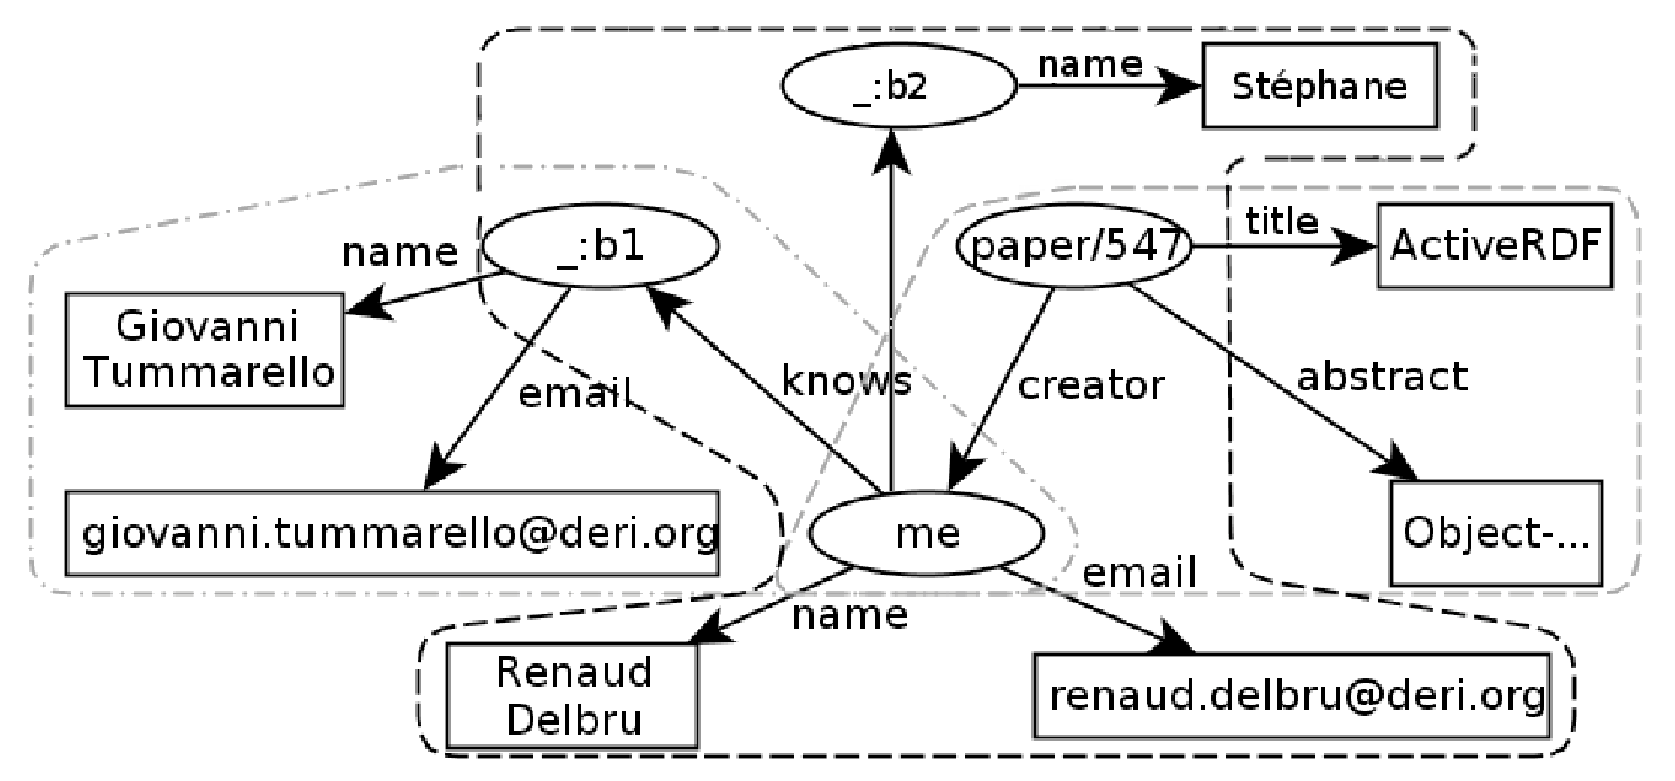
\includegraphics[scale=1]{05-ranking/figures/rdf-graph}
%	}
%	\caption{A graph divided into four entities identified by the root nodes \emph{me}, \emph{\_:b1}, \emph{\_:b2} and \emph{paper/547}.}
%	\label{fig:rdf-graph}
%\end{figure}

\section{Ranking Model Foundations}

We describe in this section vocabulary terms that will be reused throughout this chapter. We consider here a dataset to be a collection of entities, each entity being a graph. An entity may represent a person, a place, or an organisation. The \emph{unit of information} which is retrieved and ranked is an entity.

We consider an entity to be a graph centered around a node, that we call the root, where each edge provides some description of that node. We define a rooted entity as the \emph{entity description} (Definition~\ref{def:entity-description}) of a \emph{root} node, where every node in the entity description is reachable from that root node.

\begin{definition}[Rooted Entity]
Let $G = \left\langle V, A, l_V \right\rangle$ be a graph, and let $\gls{edesc}(u \in V) \subseteq A$ be the entity description of the node $u$. We call the entity description \gls{edesc}(u) a rooted entity in $u$ if and only if there is a path from $u$ to every node in $\gls{edesc}(u)$.
\end{definition}

Figure~\ref{fig:entities} depicts four entities identified by the root nodes \emph{me}, \emph{\_:b1}, \emph{\_:b2} and \emph{paper/547}.

\begin{figure}
	\centering
	\resizebox{0.65\textwidth}{!}{
		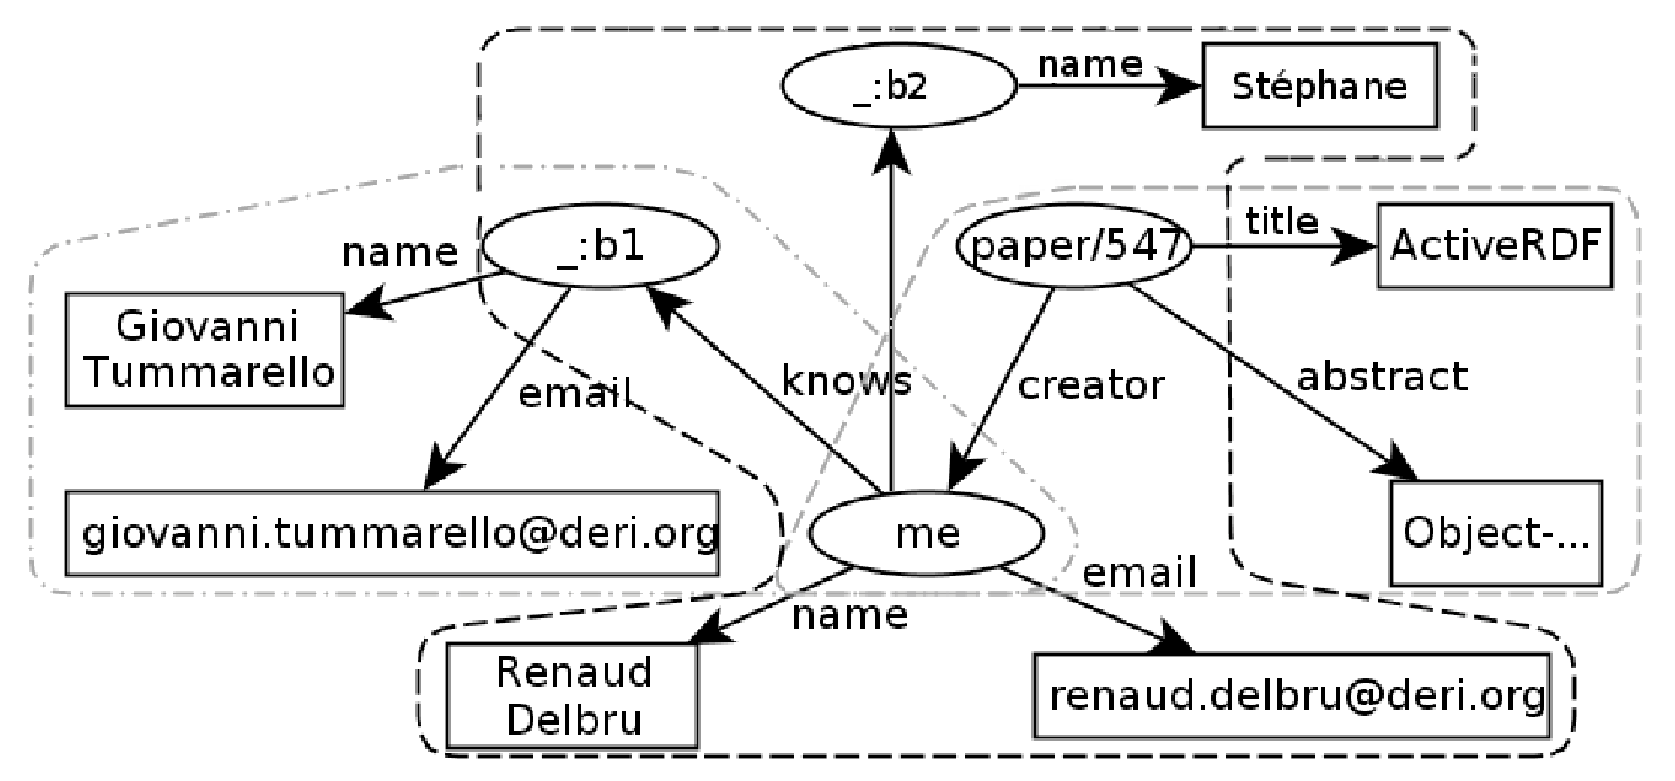
\includegraphics[scale=1]{05-ranking/figures/rdf-graph}
	}
	\caption{A graph divided into four entities identified by the root nodes \emph{me}, \emph{\_:b1}, \emph{\_:b2} and \emph{paper/547}.}
	\label{fig:entities}
\end{figure}

We define here some vocabulary used in the rest of the chapter:
\begin{description}
	\item[term:] a node label can be split over some character, e.g., a white space; we refer to a token resulting from this operation a \emph{term}.
	\item[length:] the length denotes the number of terms, e.g., in a node.
\end{description}

\section{Field-Based Ranking Models}
\label{sec:ranking-wod}

In this section, we explain how to adapt two existing field-based ranking frameworks to the graph model described in Chapter~\ref{chap:ssd}.
A field-based ranking model views a graph as composed of multiple normalized weighted fields. For example, a field can be the title, the author or the body of the document.\\

In the Probabilistic Relevance Framework~\cite{Robertson:2009:PRF} (PRF), BM25F~\cite{zaragoza:2004:microsoft} is a field-based ranking function popular for web search.
The Divergence From Randomness~\cite{amati:2002:acm} (DFR) framework gives birth to many ranking models, in particular to PL2F~\cite{macdonald:2005:clef} which is of the field-based family.\\

In field-based ranking approaches, different parts of the entity description are arranged into various categories that we denote as \emph{fields}. A field is then composed of field labels and/or edge labels. A \emph{score} of the entity is computed to reflect how relevant the entity is with regards to a query; the score computation is dependent of the fields.

In presence of a multi-valued attribute, the common approach is to merge the content of all the values into one single value.

\minisec{Ranking Features}

The following features are used in the field-based ranking functions:
\begin{labeling}{\textbf{average field length}}
	\item[\textbf{field length}] refers to the number of terms in a node label. In case of a multi-valued fields, it refers to the number of terms across all the nodes associated with the field.
	\item[\textbf{average field length}] is equal to the mean of \emph{field length} across entities.
\end{labeling}

\minisec{Normalised Term Frequency}

The ranking models presented here are from the \emph{TF-IDF} family, where \emph{TF} is a function of the term frequency, and \emph{IDF} is a function of inverse document frequency.

The intuition behind TF is that it captures the relevancy of a term within a graph, e.g., the more a term occurs in a graph, the more important it is for that graph.

In contrary, the intuition behind IDF is to capture the importance of a term within the dataset: the more a term occur in the dataset, the less relevant it is. For example, the term ``food'' would occur frequently in a cooking recipes book, however it may not be an interesting feature in a ranking function.\\

In general, the term frequency is not used ``as is'' in the TF function: it is first \emph{normalised} before applying the TF function. Term frequency normalisation is useful in cases where the length of a graph varies across the dataset: it allows to capture this variability into the ranking function, making the score of entities description comparable. In field-based ranking functions, the term frequency is normalized at the field level, capturing the length variability of a field across entities description.

\minisec{Algorithm}

Field-based ranking algorithms are constructed with the following basic operations. The importance of a query term in an entity is measured simply by how many times it occurs, i.e., its \emph{frequency}.
\begin{labeling}{\textit{\underline{Step 1:}}}
	\item[\textit{\underline{Step 1:}}] In a first step, each field of an entity is assigned a value that reflects its relevance with regards to a term in the query.
	\item[\textit{\underline{Step 2:}}] In a second step, the values of each field are summed up and a function is applied on the result so to fit the model of the ranking algorithm.
	\item[\textit{\underline{Step 3:}}] Finally, in a third step the relevance of the entity for each term in the query are summed up in order to compute the \emph{score} of the entity, which represents how important the entity is with regards to the query.
\end{labeling}

\subsection{BM25F Ranking Function}

Using the field-based ranking algorithm BM25F~\cite{zaragoza:2004:microsoft}, we show in this section how to compute the importance $Score(e,q)$ of an entity $e$ for a query $q$.\\

The first step consist in computing the normalised term frequency $\bar{f}_{t,e,a}$ with regards to the length of a field in the entity, compared to its average in the dataset.

\begin{equation}
\bar{f}_{t,e,a} = \frac{\alpha_a\times f_{t,e,a}}{1+b_a\times\left(\frac{l_{e,a}}{l_a}-1\right)}
\label{eq:bm25f_1}
\end{equation}
where:
\begin{itemize}
	\item $t$ is a term in the query $q$;
	\item $f_{t,e,a}$ is the frequency of the term $t$ in the field $a$ of the entity $e$;
	\item $\alpha_a$ is a weight of the field $a$;
	\item $b_a$ is the normalisation parameter for the field $a$ with $b_a \in \left[0,1\right]$;
	\item $l_{e,a}$ is the \emph{field length} of the attribute $a$ in the entity $e$; and
	\item $l_a$ is the \emph{average field length} of the attribute $a$.\\
\end{itemize}

In a second step, we sum up the \emph{normalised} term frequency from all fields, which result is passed to the \emph{saturation} function. It is called the ``saturation'' function because it ensures that a term occurring many times in the entity does not out-weight the importance of other query terms.

\begin{equation}
tfn_e = \frac{\sum_{a \in e}{\bar{f}_{t,e,a}}\times(k_1+1)}{\sum_{a \in e}{\bar{f}_{t,e,a}}+k_1}
\label{eq:bm25f_2}
\end{equation}
where $k_1$ is the saturation parameter.\\

In a third step, we combine the contribution of each query term, weighted by their importance in the dataset.

\begin{equation}
Score(e,q) = \alpha_e\times\sum_{t\in q}{q_t\times tfn_e \times \omega_t}
\label{eq:tfidf-score}
\end{equation}
where:
\begin{itemize}
	\item $q_t$ is the weight of the query $q$ for the term $t$, i.e., its frequency within the query $q$;
	\item $\omega_t$ is the result of the IDF function for the term $t$; and
	\item $\alpha_e$ is a weight of the entity $e$.
\end{itemize}

The IDF function is defined as
$$
\omega_t=1+log\left(\frac{N}{N_t+1}\right)
$$
where $N$ is the total number of entities in the dataset and $N_t$ is the total number of entities that have occurrences of the term $t$.

\subsection{PL2F Ranking Function}

The Divergence From Randomness (DFR) is a framework for creating ranking models. A model in the DFR framework are based on the combination of three components:
\begin{enumerate}
	\item the information gain;
	\item the randomness model; and
	\item the term frequency normalisation model.
\end{enumerate}

Using PL2F~\cite{macdonald:2005:clef} we show in this section how to compute the importance $Score(e,q)$ of an entity $e$ for a query $q$.\\

In the first step, the term frequency normalisation model used is the\emph{normalisation 2F}. Given a query term $t$ in the entity $e$, this model is a per-field normalisation of the term frequency and is defined as follows:
\begin{equation}
	\bar{f}_{t,e,a} = \alpha_a\times f_{t,e,a} \times log_2\left(1+c_a\times\frac{l_a}{l_{e,a}}\right)
	\label{eq:pl2f}
\end{equation}
where:
\begin{itemize}
	\item $t$ is a term in the query $q$;
	\item $f_{t,e,a}$ is the frequency of the term $t$ in the field $a$ of the entity $e$;
	\item $\alpha_a$ is a weight of the field $a$;
	\item $c_a$ is a per-field parameter with $c_a \in\;]0,+\infty[$;
	\item $l_{e,a}$ is the \emph{field length} of the attribute $a$ in the entity $e$; and
	\item $l_a$ is the \emph{average field length} of the attribute $a$.\\
\end{itemize}

In the second step, we apply the other two components of PL2F over the sum $tfn_e$ of the normalised term frequency across fields, i.e., $tfn = \sum_{a \in e}{\bar{f}_{t,e,a}}$:
\begin{labeling}{\underline{randomness model:}}
	\item[\underline{information gain:}] the Laplace after-effect model $P_{risk}$ is used to estimate the information gain $1-P_{risk}$:
	\begin{equation}
		P_{risk} = \frac{tfn_e}{1+tfn}
		\label{eq:dfr-prisk}
	\end{equation}

	\item[\underline{randomness model:}] the Poisson distribution $P_P$ is used to model the randomness:
	\begin{equation}
		P_{P} = \frac{\lambda^{tfn_e}}{tfn!}\times e^{-\lambda} \:\text{ where }\: \lambda=\frac{F}{N}
		\label{eq:dfr:rand-poisson}
	\end{equation}
	where $F$ is equal to the frequency of the term $t$ in the dataset, and $N$ the number of entities in the dataset.
	The factorial is approximated with the Stirling's formula:
	$$
	tfn_e!=\sqrt{2\pi}\times tfn^{tfn+0.5}\times e^{-tfn}
	$$
\end{labeling}

The weight $w_{e,t}$ of the query term $t$ in the entity $e$ is computed by combining the three components:
\begin{equation}
	w_{e,t} = \left(1-P_{risk}\right) \times \left(-log_2\left(P_{P}\right)\right)
	\label{eq:dfr-term-weight}
\end{equation}

In the third step, we combine the weight of each query term for the entity to compute the score $Score(e,q)$:
\begin{equation}
	Score(e,q) = \alpha_e\times\sum_{t\in q}{qtw \times w_{e,t}}
	\label{eq:dfr-score}
\end{equation}
where $qtw=\frac{q_t}{q_{t,max}}$ is the weight of the query $q$ for the term $t$ with $q_{t,max}$ the maximum of $q_t$ in $q$.
